%% Requires compilation with XeLaTeX or LuaLaTeX
\documentclass[10pt,xcolor={table,dvipsnames},t]{beamer}
\usetheme{diapo}
\usepackage{amsmath}

\title[Lorenz]{Data assimilation for the Lorenz system}
\subtitle{Presentation (version 0)}
\author[name]{AYDOGDU Melissa, LECOURTIER Frédérique}
\institute{\large Strasbourg University}
\date{05 april 2022}

\useoutertheme{miniframes}

\begin{document}
	
	\begin{frame}
		\titlepage
	\end{frame}
	
	\AtBeginSection[]{
		\begin{frame}
			\vfill
			\centering
			\begin{beamercolorbox}[sep=5pt,shadow=true,rounded=true]{subtitle}
				\usebeamerfont{title}\insertsectionhead\par%
			\end{beamercolorbox}
			\vfill
		\end{frame}
	}


\section{Data assimilation }
	\begin{frame}{Introduction to the data assimilation}
	    Data assimilation is widely used in:
	    \begin{enumerate}[\textbullet]
			\item weather forecastinf
			\item ocean simulation
	    \end{enumerate}	 
    	The main idea of the data assimilation is to combine:
	    \begin{enumerate}[\textbullet]
			\item a model
			\item some observations
	    \end{enumerate}	 
	    The best estimate is searched for as a linear combination of the background estimate and the observations:
	    $$x^a=Lx^b+Ky^0$$
	    with $x^a$ the analyzed state, $x^b$ the state of the model and $y^0$ the observations.
	\end{frame}
	\begin{frame}
	    Data assimilation methods are often split into two families:
	    \begin{enumerate}[\textbullet]
			\item statistical method
			\item variational method
    	\end{enumerate}
	\end{frame}
\section{statistical approach}
    \begin{frame}{Kalman filter}
        The Kalman filter method consists in looking for $x^a$ an analysis, this analysis will be a linear combination of what we already know, our model and our observations.
        $$x^a=x^b+K(y-x^b)$$
        with K the gain matrix.
        To simplify let’s consider that we are in 1D, and we suppose that the true state $x^t$ exists:
        $$x^a-x^t=x^b-x^t+K(y-x^t-x^b+x^t)$$
    \end{frame}   
    \begin{frame}
        We will therefore have errors such as:
        $$\begin{aligned}
            &\epsilon^a=x^a-x^t, \\
            &\epsilon^b=x^b-x^t, \\
            &\epsilon^y=y-x^t, \\
        \end{aligned}$$
        If we have many realisation of these error, then we can write:
        $$<\epsilon^a>=<\epsilon^b>+K(<\epsilon^y>-<\epsilon^b>)$$
        We want to have the analysis error variance as low as possible .So we want to minimize $<(\epsilon^a)^2>$ with respect to $K$ :
        $$<(\epsilon^a)^2>=<(\epsilon^b)^2>+K^2<(\epsilon^y-\epsilon^b)^2>+2K<\epsilon^b(\epsilon^y-\epsilon^b)^2>$$
    \end{frame}
    \begin{frame}
        We assume that the errors in the background and observation are uncorrelated.
        $$K=\frac{<(\epsilon^b)^2>}{<(\epsilon^b)^2>+<(\epsilon^y)^2>} \Rightarrow K=\frac{(\sigma^b)^2}{(\sigma^b)^2+(\sigma^y)^2} $$
        where $(\sigma^y)^2$ is the observation error variance and $(\sigma^b)^2$ is the background or model error variance.
        \newline If  $(\sigma^y)^2=0$, $K=1$ and $x^a=y$ => observation are perfect.
        \newline And if $(\sigma^b)^2=0$, $K=0$ and $x^a=x^b$ => we ignore the observations.
    \end{frame}
    \begin{frame}
        Now that we have explained the method for finding $x^a$ let's try to generalize our formula in a multi-dimensional case.

        $$\left\{\begin{aligned}
		    &x^a=(I-KH)x^b+Ky^0=x^b+K(y^0-H(x^b)) \\
            &K=BH^T(HBH^T+R)^{-1} \\
	    \end{aligned}\right.$$
        With $K$ the gain or weight matrix.
        This formulation is called the Best Linear Unbiased Estimator (BLUE).
    \end{frame}
    \begin{frame}
        \pgfimage[height=5.5cm,width=11cm]{images/schema_kalman_filter.png}
    \end{frame}
\section{Variational approach}
    \begin{frame}{Minimizing a cost function}
        Solves the analysis problem through an optimisation (minimisation of a cost-function)
        Variational approach of BLUE consists in finding $x^a=\arg\max_{x}J$:
        $$\begin{aligned}
            J(x)&=\frac{1}{2}(x^b-x)^TB^{-1}(x^b-x)+\frac{1}{2}(y-H(x))^TR^{-1}(y-H(x)) \\
            &=\frac{1}{2}\|x-x^b\|_B^2+\frac{1}{2}\|H(x)-y^0\|_R^2
        \end{aligned}$$
    \end{frame}
    \begin{frame}
        \pgfimage[height=5.5cm,width=11cm]{images/schema_3D_Var.png}
    \end{frame}
\section{Ensemble filter kalman}
    \begin{frame}{Ensemble Filter Kalman}
        The ENKF method consists in using the Kalman filter method in high dimension and compare P by a set of states $x_1,x_2,..,x_{m}$. So we can approximate the moments of the error by the moments of the sample.
        The we have:
        $$x_i^a=x_i^f+K[y-h(x_i^f)]$$
        with $h(x_i^f)$ the observation operator.
        We can also define the Kalman gains: 
        $$K=P^f H^T(HP^f H^T+R)^{-1}$$
        To begin with we can estimate the
        forecast error covariance matrix as:
        $$P^f=\frac{1}{m-1}\sum_{i=1}^{m}(x_i^f-\bar{x}^f)(x_i^f-\bar{x}^f)^T~~\text{with}~~\bar{x}^f=\frac{1}{m}\sum_{i=1}^{m}x_i^f $$ .
    \end{frame}
\section{Presentation of the results}
    \begin{frame}{Harmonic oscillator}
        $$\qquad \frac{\partial x}{\partial t}=v \quad \Rightarrow \quad \frac{\partial^2 x}{\partial t^2}=\frac{\partial v}{\partial t}$$
        \begin{enumerate}[\textbullet]
			\item We choose for the initial point $(2,0)$
			\item For the period let's take Pe=$\frac{2\pi}{w}$ with $w$ the first components of our initial point
			\item For the discretisation,  dt=$\frac{\text{Pe}}{20}$ 
			\item We try to find the solution in the interval $[0,T]$ with T=$3\text{Pe}$
    	\end{enumerate}
    \end{frame}
    \begin{frame}
        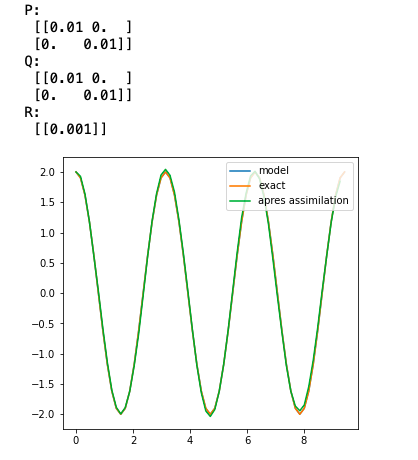
\includegraphics[width=0.3\textwidth]{"images/oscillator1.png"}
		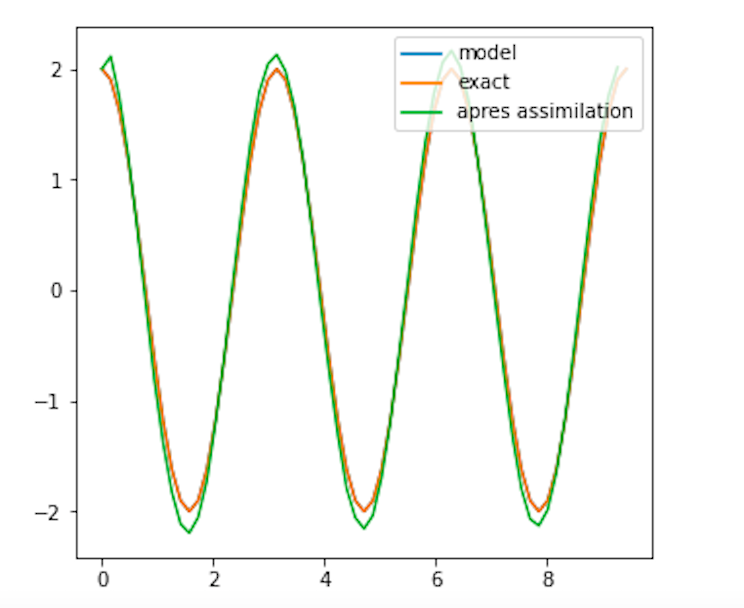
\includegraphics[width=0.3\textwidth]{"images/oscillator2.png"}
		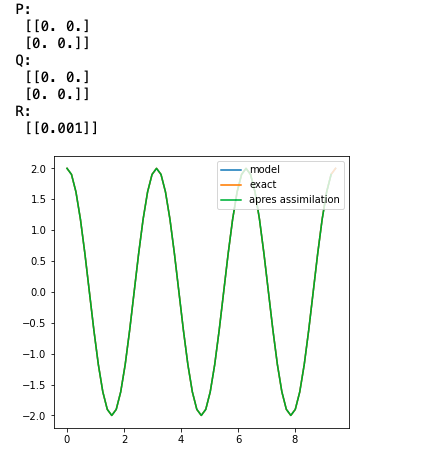
\includegraphics[width=0.3\textwidth]{"images/oscillator3.png"}
        
    \end{frame}
    \begin{frame}{Lorenz System}
        \begin{enumerate}[\textbullet]
			\item  $(\sigma, r, b)=(12.,6.,12.)$,
			\item Initial point $x=(-10.,-10.,25.)$,
			\item For the interval we choose [0,T] with T=1,
			\item Let's take 
			$$P=\begin{pmatrix}
            0.1 & 0. & 0. \\
            0. & 0.1 & 0. \\
            0. & 0. & 0.1 \\
            \end{pmatrix} ,
            Q=\begin{pmatrix}
            0.1 & 0. & 0. \\
            0. & 0.1 & 0. \\
            0. & 0. & 0.1 \\
            \end{pmatrix},
            R=\begin{pmatrix}
            0.01 & 0. & 0. \\
            0. & 0.01 & 0. \\
            0. & 0. & 0.01 \\
            \end{pmatrix}.$$ 
    	\end{enumerate}
    \end{frame}
    \begin{frame}
       \pgfimage[width=\linewidth]{images/lorenz_1.png} 
    \end{frame}
    \begin{frame}
        \begin{enumerate}[\textbullet]
			\item  For the model $(\sigma, r, b)=(10.,6.,10.)$,
			\item For the observation $(\sigma, r, b)=(12.,6.,12.)$,
			\item Initial point $x=(-10.,-10.,25.))$,
			\item we take a time step of 0.1s
			\item For the interval we choose [0,T] with T=4,
			\item Let's take for the fist case
			$$P=\begin{pmatrix}
            0.1 & 0. & 0. \\
            0. & 0.1 & 0. \\
            0. & 0. & 0.1 \\
            \end{pmatrix} ,
            Q=\begin{pmatrix}
            0.01 & 0. & 0. \\
            0. & 0.01 & 0. \\
            0. & 0. & 0.01 \\
            \end{pmatrix},
            R=\begin{pmatrix}
            0.1 & 0. & 0. \\
            0. & 0.1 & 0. \\
            0. & 0. & 0.1 \\
            \end{pmatrix}.$$ 
            \newline For the second case lets take :
            $$P=\begin{pmatrix}
            0.1 & 0. & 0. \\
            0. & 0.1 & 0. \\
            0. & 0. & 0.1 \\
            \end{pmatrix} ,
            Q=\begin{pmatrix}
            0.1 & 0. & 0. \\
            0. & 0.1 & 0. \\
            0. & 0. & 0.1 \\
            \end{pmatrix},
            R=\begin{pmatrix}
            0.01 & 0. & 0. \\
            0. & 0.01 & 0. \\
            0. & 0. & 0.01 \\
            \end{pmatrix}.$$ 
    	\end{enumerate}
    \end{frame}
    \begin{frame}
        \pgfimage[width=\linewidth]{images/lorenz_2.png} 
        \pgfimage[width=\linewidth]{images/lorenz3_b.png} 
    \end{frame}
\end{document}
	